\documentclass[a4paper,10pt,fleqn]{article}
\usepackage{fullpage}
\setlength{\mathindent}{0pt}

% do not indent first line of paragraph.
\setlength{\parindent}{0cm}
% But separate them with 3-10mm
\setlength{\parskip}{6mm plus4mm minus3mm}

\usepackage[dutch]{babel}
\usepackage[utf8]{inputenc}

%~ \usepackage{fullpage}
%~ \usepackage[official]{eurosym} % depens on: texlive-fonts-recommended
\usepackage{amsmath}
\usepackage{amssymb}
%~ \usepackage{tabularx}

% Hyperref package, clickable internal links.
% colorlinks to remove ugly boxes around links...
% \usepackage[colorlinks]{hyperref}

\makeatletter
\newcommand*{\centerfloat}{%
  \parindent \z@
  \leftskip \z@ \@plus 1fil \@minus \textwidth
  \rightskip\leftskip
  \parfillskip \z@skip}
\makeatother

\usepackage{enumerate}

\usepackage{subfigure}
\usepackage{pgf}
\usepackage{tikz}
\usetikzlibrary{arrows,automata}

\title{TI2736-A\\ Assignment 1:  Artificial Neural Network}

\author{
	David Akkerman - 4220390 \\
	Jan Pieter Waagmeester - 1222848 \\
}

\begin{document}
\maketitle
{\small Onze groepssgenoot is om persoonlijke redenen gestopt met het vak. Deze opdracht hebben we met ons tweeën gemaakt.}

\begin{enumerate}[1.]
	% 1. How many input neurons are needed for this assignment?
	\item Omdat er 10 eigenschappen zijn hebben we 10 inputneurons nodig.

	% 2. How many output neurons do you require?
	\item Voor de 7 verschillende classes hebben we 7 outputneurons nodig.

	% 3. How many hidden neurons will your network have? (Give an initial guess, later you will try different number of hidden neurons and analyze the network’s performance).
	\item We beginnen met 10 hidden neurons.

	% 4. Which activation function(s) will you use?
	\item We zullen de sigmoid-functie gebruiken:
	$$Y^{sigmoid} = \left( \frac{1}{1 + e^{-X}} \right)$$

	%5. Give a schematic diagram of your complete network
	\item Ons netwerk kan voorgesteld worden als in het volgende plaatje, in dit geval met 10 \textit{hidden neurons}. Dit aantal kan uiteraard gevarieerd worden. \\

	\begin{center}
		\tikzstyle{neuron}=[draw=black!50,minimum size=20pt,inner sep=3pt]
		\tikzstyle{input}=[rectangle]
		\tikzstyle{hidden}=[circle]
		\tikzstyle{output}=[circle]
		\tikzstyle{connection}=[draw=black!40, very thin]

		\begin{tikzpicture}[node distance=3cm,scale=1,auto]
			\def \scalar {0.9}

			\def \inputs {10}
			\def \hidden {10}
			\def \outputs {7}

			\foreach \m in {1,...,\inputs}{
				\node[neuron,input] (input-\m) at(0, {(-\m + \inputs / 2) * \scalar}) {$\m$};
			}

			\foreach \m in {1,...,\hidden}{
				\node[neuron,hidden] (hidden-\m) at(7, {(-\m + \hidden / 2) * \scalar}) {$\m$};
			}

			\foreach \m in {1,...,\outputs}{
				\node[neuron,output] (output-\m) at(14, {(-\m + \outputs / 2) * \scalar}) {$\m$};
			}

			% connections between neurons
			\foreach \j in {1,...,\hidden}{
				% input to hidden layer
				\foreach \i in {1,...,\inputs}{
					\path (input-\i) edge [connection] (hidden-\j);
				}
				% hidden to output layer
				\foreach \k in {1,...,\outputs}{
					\path (hidden-\j) edge [connection] (output-\k);
				}
			}


			% calculate the lowest Y of the three label positions and put each label there.
			\pgfmathparse{(-max(\inputs, \hidden, \outputs) / 2 - 1) * \scalar}
			\edef\labelY{\pgfmathresult}

			\node (input) 	at (0, \labelY)				{inputs};
			\node (wij)   	at (3.5, \labelY + 0.5)		{$w_{ij}$};
			\node (hidden)	at (7, \labelY)				{hidden};
			\node (wjk)		at (10.5, \labelY + 0.5)	{$w_{jk}$};
			\node (output) 	at (14, \labelY)			{outputs};
		\end{tikzpicture}
	\end{center}

    % 2.2 Training
	% 6. How and why did you divide your data into a training, validation and test set?
	\item We gebruiken ongeveer $50\%$ van de data voor training, $25\%$ voor validatie en $25\%$ als testset. De data lijkt aardig random gesorteerd te zijn, het is dus niet nodig om te zorgen dat er ongeveer even veel van elke class in elke set aanwezig is.

	% 7. How do you evaluate the performance of your network?
	\item Door te kijken naar de \textit{Mean square error} (MSE) op te trainingset, en op de validatieset. Zolang ze beide dalen, wordt het netwerk beter. Als de MSE op de trainingsset daalt, maar die op de validatieset gaat stijgen is er sprake van overfitting: het netwerk wordt beter in het herkennen van ruis in de trainingsset, maar niet beter in het herkennen van de algemene patronen.

	% 8. When and why do you decide to end the training?
	\item Op het moment dat het netwerk overtrained dreigt te raken, dus wanneer de MSE niet langer daalt en en begint te stijgen, wordt de training gestopt, zodat het nog wel geschikt is voor andere data dan de trainingsset. Daarnaast is het handig voor de snelheid van het netwerk te stellen dat wanneer de MSE van het netwerk over tien epochs niet meer dan 0.1\% verschilt, ook het trainingsproces te beëindigen. Gebeurt dit niet, dan kan het nog erg lang doorgaan met optimaliseren, zonder dat er in het uiteindelijke resultaat verschil merkbaar is.

	% 9. Train your network 10 times, each with different initial weights. How does the initialization impact the performance?
	\item Wanneer het netwerk tienmaal getraind wordt, komt hij iedere keer redelijk op dezelfde waarde voor de MSE uit. Slechts eenmaal laat hij een totaal andere curve zien. Dit komt waarschijnlijk doordat de geïnitialiseerde waardes van de gewichten en vergelijkingswaarden ver van een lokaal optimum liggen. Aan de andere lijnen valt te zien dat de meeste lokale optima dicht bij elkaar in de buurt liggen.
    \begin{figure}[!ht]
    	\centerfloat
        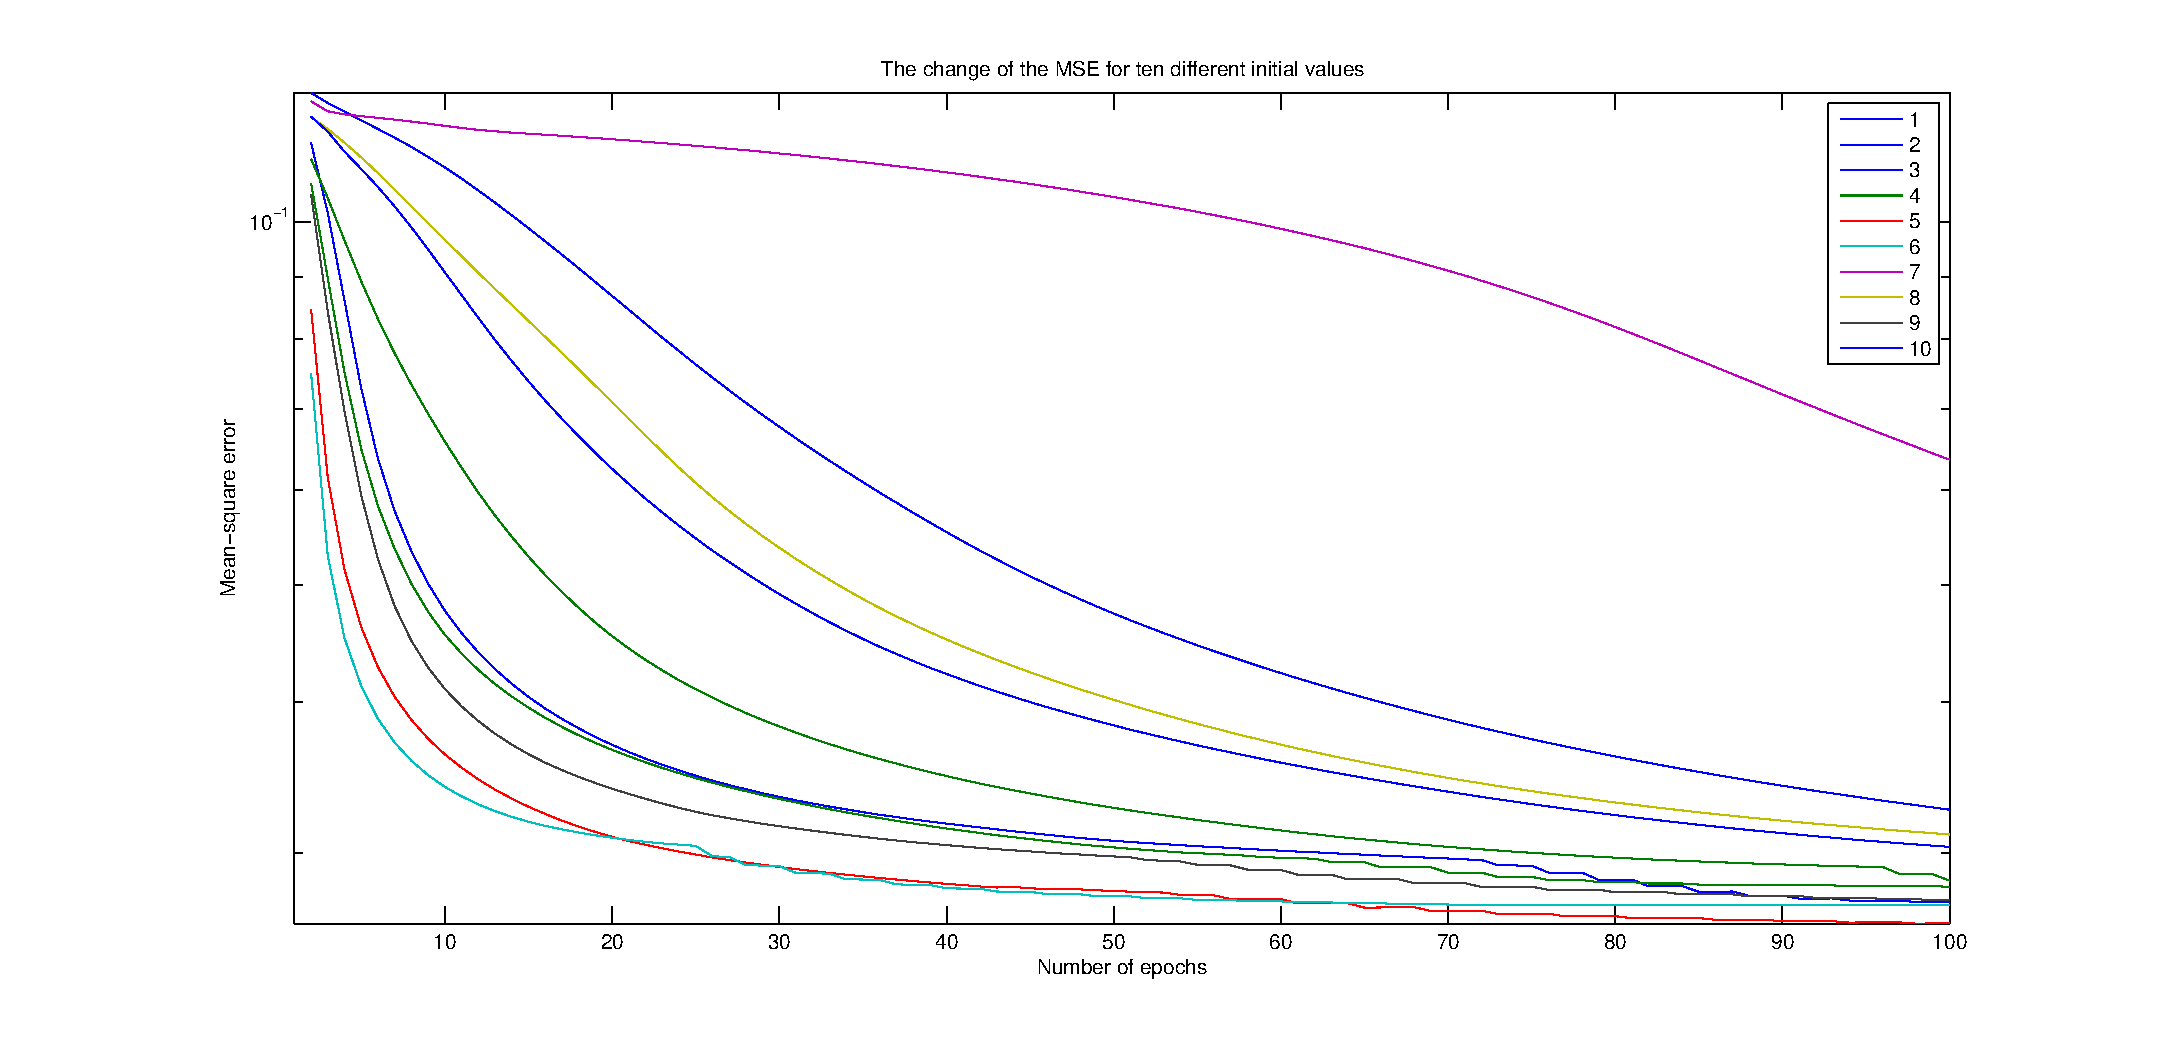
\includegraphics[width=1.35\textwidth]{images/train-10-times-learning_rate}
    \end{figure}

    \pagebreak
	% 2.3 Optimization
	% 10. Train your network with different amounts of hidden neurons. At least 3 times chosen within the range of 7-30 hidden neurons. Generate a plot of the final performance versus the number of hidden neurons in the network. (Hint: you can use the MATLAB command ❜boxplot' or 'errorbar' )
	\item We hebben 23 verschillende netwerken, met 7 - 30 \textit{hidden neurons} 10 keer getraind. De succes-ratio van die netwerken hebben we verwerkt in de volgende boxplots:
    \begin{figure}[!ht]
    	\centering
        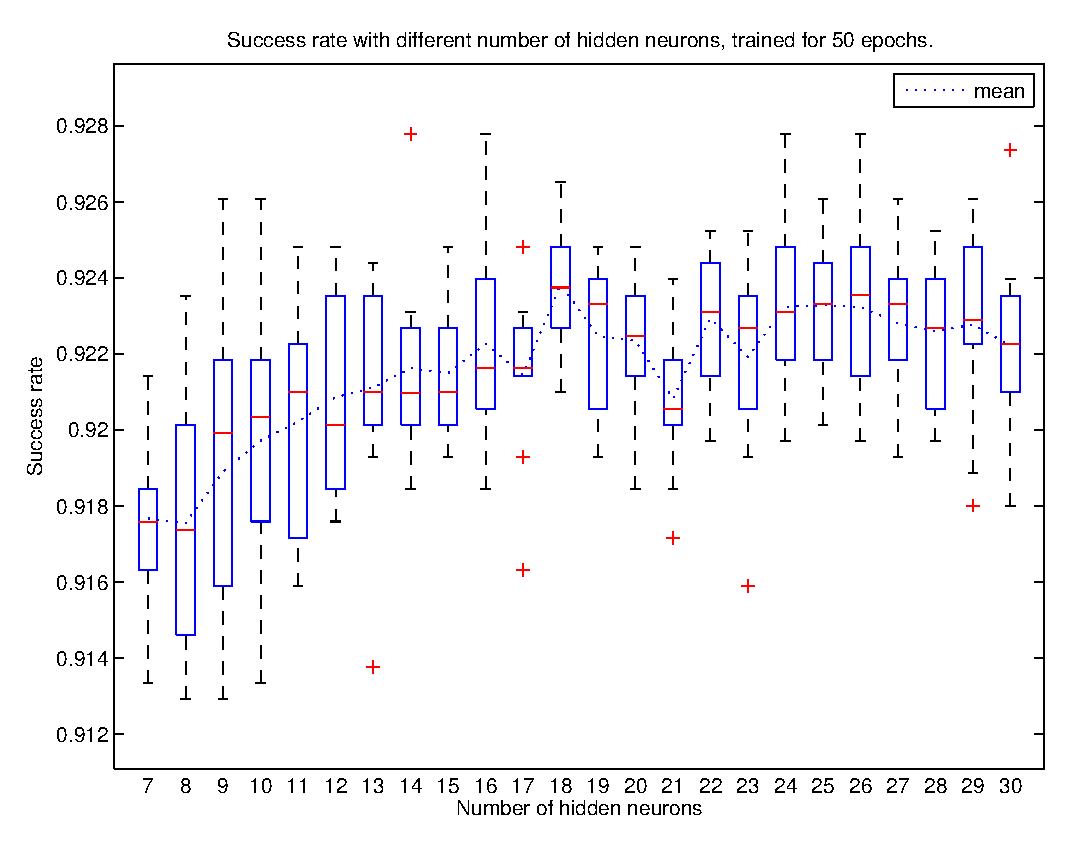
\includegraphics[width=1\textwidth]{images/error-boxplot}
    \end{figure}
    Hieruit blijkt ondermeer dat de performance ook bij een klein aantal \textit{hidden neurons} nog best goed is. Naast dit plaatje hebben we nog gekeken naar kleinere aantallen en zelfs met 4 \textit{hidden neurons} wordt in gemiddeld $85\%$ van de gevallen nog een correcte indeling in klassen gemaakt.

    Verder is duidelijk dat het op een gegeven moment geen zin meer heeft om nog meer \textit{hidden neurons} toe te voeggen, het resulterende netwerk heeft er geen significant betere performance door.

    Wat ook interessant is om bij grotere aantallen neuronen te kijken naar de gewichten $w_{ij}$ en $w_jk$. Dat kan bijvoorbeeld met \verb|imagesc|. Er blijkt dan dat een deel van de neuronen bijna niet meer mee doet in de berekening van de output. Helaas is er in dit verslag geen ruimte voor plaatjes hiervan, laat staan voor een animatie van de plaatjes gedurdende de training.

    \pagebreak
	% 11. Pick the architecture with the best result and show a plot of the performance of the training set and the validation set during training, across epochs.
	\item Hier een afbeelding van een netwerk met 19 \textit{hidden neurons}. In de voorgaande boxplot kwam 18 hidden neurons beter uit de bus, maar dit was de beste prestatie uit een groot aantal runs en het netwerk wat we gebruikt hebben om de class van de set \verb|unknown.txt| te bepalen.
	\begin{figure}[!ht]
    	\centering
        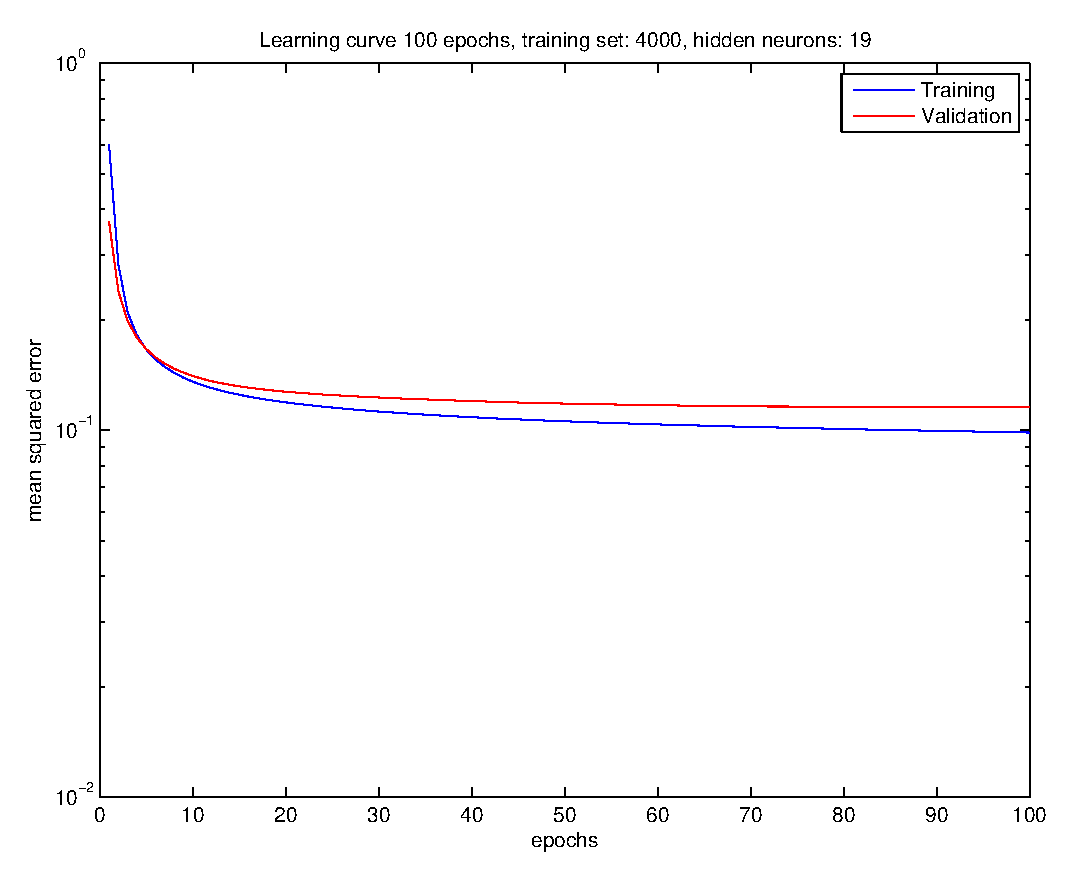
\includegraphics[width=.8\textwidth]{images/learning_curve}
    \end{figure}

    	% 2.4 Evaluation
	% 12. What is the success rate of your network on the test set? How does it compare to the results of the validation set?
	\item De \textit{success rate} van de testset is 0.91 $\pm 0.01$. Dit is vergelijkbaar met die van de validatieset. Het netwerk wordt echter wel geoptimaliseerd met behulp van de \textit{success rate} van de validatieset door de training te stoppen op het moment dat deze weer stijgt. Dit heeft ook een positief effect op de \textit{success rate} van de test set, maar het kan net buiten het optimum liggen. Dit is echter verwaarloosbaar in vergelijking met de verschillen tussen verschillende trainingsrondes.

	% 13. Show a confusion matrix of your test set. How should it be read? Where did your network make the most mistakes? (Search for the meaning and purpose of a confusion matrix and use the function 'plotconfusion' from MATLAB).
	\item Een confusionplot gemaakt met \verb|plotconfusion| (zie volgende pagina). Op de $y$-as staan de output-classes zoals ons netwerk produceert. Op de $x$-as staat de verwachtingswaarde. Een juist voorspelde waarde staat dus op de diagonaal, in de groene cellen.  \\
    Verder is er ook uit af te lezen dat in dit geval het netwerk 20 keer een 4 voorspelde, terwijl het een 7 had moeten zijn. Dat is een duidelijke uitschieter waar verder voornamelijk fouten onder de 10 staan.

	\begin{figure}[!ht]
    	\centering
        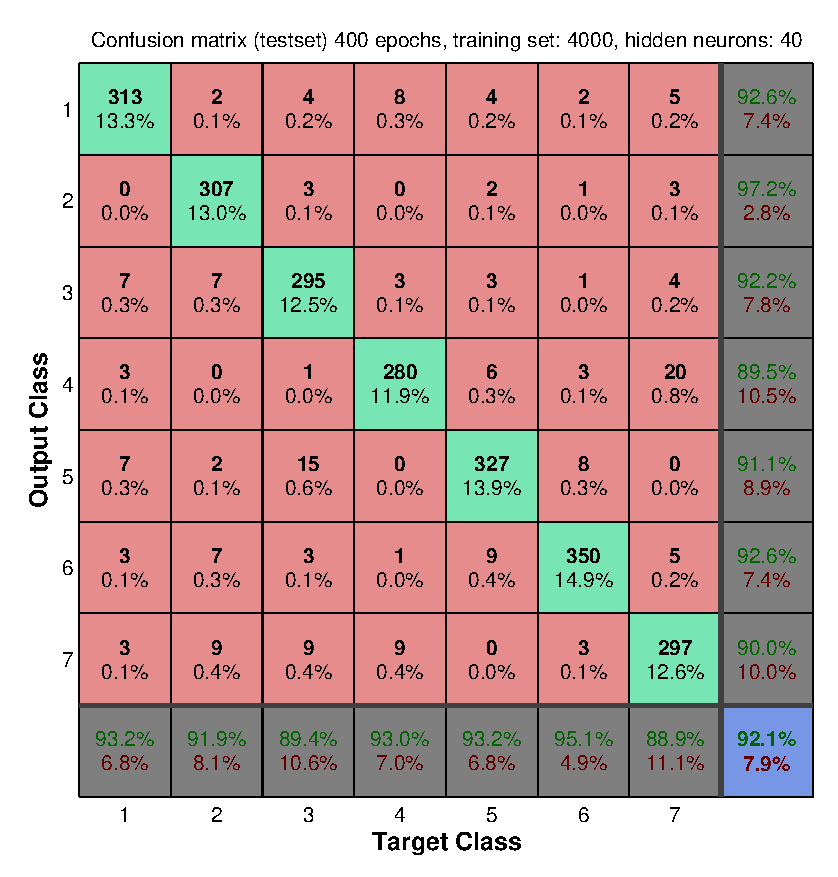
\includegraphics[width=.65\textwidth]{images/confusion-matrix-eps}
    \end{figure}

	% 14. Feed the unknown set (provided on Blackboard) to the network. Export the resulting classes as a comma-separated file exactly as detailed in section 1.2.
	\item Geüpload naar blackboard als \verb|5_classes.txt|


	\pagebreak
	% 2.5 Matlab's Toolbox
	% 15. Use the Toolbox to create a network similar to the one you’ve just made. (You can start the toolbox GUI with 'nnstart' or directly go to pattern recognition with 'nprtool').
	\item Met \verb|nprtool| is het binnen een paar minuten mogelijk om een netwerk te maken wat er zo uitziet:

	\begin{figure}[!ht]
		\centering
		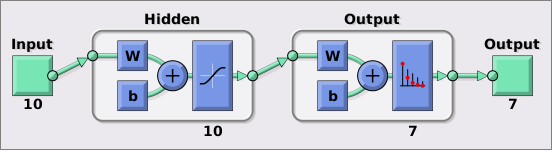
\includegraphics[width=.7\textwidth]{images/nprtool-diagram}
	\end{figure}

	% 16. Comment on the differences between your network’s performance and the Toolbox.
	\item De performance van dit netwerk is erg goed, en de training is ook erg snel klaar. Ook met 10 hidden neurons worden succes-percentages van rond de $92\%$ gehaald.

	Tijdens het maken van het eigen neurale netwerk had ik het idee dat het gebruiken van de sigmoid-activatiefunctie wellicht voor de output-layer niet handig was. Dit netwerk gebruikt een softmax activatiefunctie in de output-layer, wellicht ook een reden van betere prestaties.

	De veel hogere trainingsefficientie is waarschijnlijk verklaarbaar door bijvoorbeeld implementatie in correcte matrix-algebra en het toevoegen van het aanpassen van de \textit{learning rate}, het toevoegen van een momentum-term in de delta-rule (Negnevitsky, equation 6.17).
\end{enumerate}
\end{document}

